\documentclass[12pt]{article}

%Graphic premable
\usepackage{graphicx} %import images
\usepackage{float} % control float positions
\usepackage{caption}  
\usepackage{subcaption}

\usepackage[margin=1 in, left=1.5in, includefoot]{geometry}
\usepackage{array}
\usepackage{amssymb}
\usepackage{array}
\usepackage{amsmath}
% Header and Footer 
\usepackage{fancyhdr}
\pagestyle{fancy}
\fancyhead{}
\renewcommand{\headrulewidth}{0pt}
\renewcommand{\footrulewidth}{1pt}

% Bibliography
\usepackage{apacite}

\begin{document}

%Title
\begin{titlepage}
\begin{center} 
\Huge{\bfseries Notion $|$ AI in Strategy} \\
[1.5cm]
\huge{Project Proposal} \\
[1.5cm]
\begin{figure}[h] 
\centering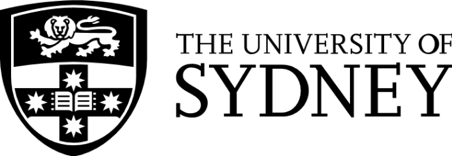
\includegraphics[width=12cm]{usyd} 
\end{figure} 
\huge{Information Technology Capstone Project\\COMP5703} \\
[3CM]
\LARGE{\bfseries Group Members} \\
[1cm]
\end{center}
\LARGE{ 1. Min Jeong Oh (470151813) \\ 2. Hongjin Qian (470141124) \\ 3. Sheng Yuan (430058318)\\4. Prerona Majumder (470531989)\\5.	Yichao Fu (460283988)}
\end{titlepage}

%Abstract
\pagenumbering{roman}
\section*{Abstract}
The objective of this project is to find underlying themes of the articles by unsupervised clustering and to find the collective sentences or phrases that define said clusters and rank them (sentences or phrases) according to their relevance to the particular cluster. Another objective is to find the interrelations between the clusters thus formed. The first step in achieving this objective is proper pre-processing which involves filtering stop words, stemming, tokenisation and finally vectorisation. Tf-idf is the basic vectorisation method but Watson NLU API provides better representations of the dataset by extracting high level features. Both these methods will be explored in the project. The most important part of this project is feature selection which will reduce the dimensions of the dataset significantly for feasible computations, all the while retaining the important features. A Deep Learning approach is proposed for feature selection by the use of Deep Autoencoders which can be integrated with the basic clustering algorithms (k-means, Gaussian Mixture, Agglomerative Clustering). A few Deep Learning methods for clustering are also proposed namely Deep Embedded Clustering (DEC) and DeepCluster which uses the architecture from the Deep Autoencoder. DEC minimises Kullback-Leibler (KL) Divergence for parameter optimisation and DeepCluster integrates clustering along with the reconstruction of input in the same iteration. Experiments will be performed with all the proposed methods to find the solution which best represents the cluster themes. 



\addcontentsline{toc}{section}{\numberline{}Abstract}
\cleardoublepage


%Table of content
\tableofcontents
\thispagestyle{empty}
\cleardoublepage



\pagenumbering{arabic}
\setcounter{page}{1}
\section{Introduction}\label{sec:intro}
With the dramatic increase in digital text documents, text mining in big data analytics is becoming increasingly significance to academic research, government, marketing and business\cite{cogburn2017introduction}. The aim of text mining is to extract the meaningful information from the unstructured information by using various algorithms, such as natural language processing (NLP) and machine learning algorithms. Text mining can help the researchers to find the hidden information and latent pattern, including identifying and developing new hypotheses, attaining knowledge and improving understanding \cite{3benefit}. \\

Our client, Notion, is an enterprise intelligence start up with large financial services clients on board. Our project is aims to develop tools for Notion to identify the themes or ideas rather than entities or concepts from the articles automatically. Moreover, the key purpose is to find the interrelations between those themes or ideas and rank the importance of them to the relevant articles. The current dataset is the articles, which were collected during the periods when the Royal Commission hearings were hold. The Royal Commission was established on 14 December 2017 by the Governor-General of the Commonwealth of Australia, His Excellency General the Honourable Sir Peter Cosgrove AK MC (Retd) and it already had 5 round hearings on Misconduct in the Banking, Superannuation and Financial Services \cite{royalcommission}. The collected articles are all related to the topics of the hearings (E.g. Framing finance and Interactions between Aboriginal and Torres Strait Islander people and financial services entities in the fourth-round hearings). By using our applications, the latent factors leading to those events can be found. \\

As a data science project, several text mining approaches will be applied. Natural language processing (NLP), a sub-field of computer science, artificial intelligence and linguistics, is designed to understand the natural language by utilizing computer \cite{allahyari2017brief}. Information extraction (IE) is process that extracting meaningful information from documents. Unsupervised Learning Methods are the techniques to find the hidden structure out of unlabelled data, including clustering and topic modelling. \\

\section{Related work/Literature Review}\label{sec:lr}
According to aim of our project, the two important parts are feature engineering and clustering techniques. To represent a text document, a large number of features are introduced, which will increase the complexity and dimensionality of the data. In order to these problems, the feature selection and extraction can be implemented. The most relevant information will be obtained to describe the original data in a lower dimensionality space with appropriate accuracy. For unsupervised learning task, clustering is one of the most popular algorithms, which can group the similar data among the collection. 
\subsection{Advantage and Disadvantage of Common Methods}
A study conducted by Hong Liang, Xiao Sun, Yunlei Sun and Yuan Gao \cite{liang2017text} introduced the common methods of text feature extraction, which contain filtration, fusion, mapping and clustering methods.  Moreover, Foram P.Shah and Vibha Patel analysed the cons and pros of important methods in feature selection and extraction\cite{shah2016review}. \\
 
Filtration method, which includes word frequency, information gain, and mutual information, is a fast and proper solution for large-scale text feature extraction. More specifically, the word frequency method aims to remove the words with the frequencies that are under a certain threshold. It has the lower cost in computation and is easy to implement. However, it has the problem that it treats the rare terms as non-informative items, which are vital in some cases. For information gain method, its evaluation is related to the entropy of each feature. The key process is to rank the features in a descending order by computing the information gain and drop the features with small information gain. Hence, it can decide the most relevant attributes but cannot eliminate redundant features. Compared with these two methods, mutual information method can measure the similarity between two variables, which is good at letting the words with the lowest rising frequency with more weight. \\
 
The commonly used methods in mapping method are latent semantic index (LSI) and principal component analysis (PCA). For LSI, it can analyse the relationship between a set of text documents and then generate a set of concepts related them. It is considered as a simple method. But as a linear model, it is not suitable to handle non-linear dependencies. For PCA, it can covert the variables into the principal components, which has lower dimensionality. It has the advantages that it is a simple technique in approximating the covariance or correlation matrix. However, the drawback is that the covariance matrix cannot be evaluated in an accurate manner. \\

\subsection{Latent Dirichlet Allocation}
Latent structure from context can be found by using topic modelling\cite{blei2003latent}. The assign of a topic can be viewed as the appearance of words belong to certain group. There are some methods of topic model like Probabilistic Latent Semantic Analysis (PLSA), Latent Dirichlet Allocation (LDA). A study found that LDA has better performance than PLSA\cite{barde2017overview}. According to the study, LDA can assign topic to a new document easily when LDA and PLSA are used on the real data.

\subsection{Link Based BPSO for Feature Selection}
Particle Swarm Optimisation (PSO) developed by Eberhart and Kennedy \cite{kennedy2011particle} is inspired by birds flocking or fish schooling. It is a robust population based algorithm which is computationally fast. It starts out with a set of initial solution called a swarm and the individual solutions are called particles. Each particle has a fitness value (usually Mean Absolute Difference) and is represented as a vector which consists of the particle’s position, its best overall position and its velocity. Another variable called the global best is associated with the whole population. These variables are adjusted according to its own experience as well as its neighbours. PSO is a continuous technique so Binary PSO (BPSO) was developed \cite{kennedy1997discrete} for binary operations where sigmoid function is used to convert from continuous form. \\

A better form of BPSO called Linked based BPSO (LBPSO) \cite{kushwaha2018link} utilises a BA model (proposed by Barabasi \& Albert) \cite{barabasi2000scale} to construct a scale free topology where at every step more particles are added to the network depending on a probability. A link function is calculated using a link matrix which evaluates the relationship between two particles. The algorithm also uses a Crossover Operator and a Mutation Operator \cite{bolaji2016comprehensive}. These PSO algorithms are then integrated with Clustering algorithms like k-means to enhance the classification performance giving higher accuracy. \\

\subsection{Deep Learning Methods}
The traditional feature extraction methods are required hand-crafted features. However, for the methods in deep learning area, there is no need for human engineers to design the features. Instead of it, these methods can learn the features from the original data automatically\cite{liang2017text}. The approaches contain auto-encoder, convolutional neural network (CNN), recurrent neural network (RNN) and so on.\\
 
 
Auto-encoder is a feedforward neural network and used in unsupervised manner\cite{oshri2016there}, which aims to compress the data into a short code. According to the article of Barak Oshri and Nishith Khandwala, they did an experiment by using different types of autoencoders, such as basic encoder, RNN encoder and CNN encoder, to transform the word vectors into a summary vector. The aim of the experiment is to find the effective semantic representations of variable size text. After training their models with 10,000 sentences from Wikipedia, the results showed that the CNN Encoder had the highest score of reconstruction.\\

\subsection{Deep learning Methods of Clustering}
K-means and GMM are two popular clustering algorithm and have widely used in many applications. But both methods perform badly when input data are in high-dimensional space. Deep Embedded Clustering (DEC) is a method proposed by Xie ( (Junyuan Xie, 2016) which starts by mapping original feature space to low-dimensional space and then perform cluster with the latent feature space. Inspired by DEC, another method DeepCluster was proposed by Kai (Tian, 2016), which is based on the same deep network structure as Xie but combines both deep network and clustering algorithm together. Both methods have conducted experiments based on image dataset( MNIST, USPS) and text dataset (Reuters 10K) and reached state-of-the-art accuracy.




\section{Project Problems}\label{sec:pp}
\subsection{Project Aims \& Objectives}
The main goal of this project is providing a better way of solving problems for our client, Notion. Notion is an enterprise intelligence company that generates key insight from tens of thousands of lines of text data and provides information that can help their clients’ strategic decisions. \\

The company is currently working on a project to analyse the text data from The Royal Commission into Misconduct in the Banking, Superannuation and Financial Services Industry. The Commission invite individuals or entities to make public submissions. Then, The Commission is required to conduct an inquiry although it cannot resolve individual disputes. The first round of public hearing  commenced on 13 March 2018, and four more rounds have been held since then. \\

Notion is aiming to discover the underlying structure of the text data of The Royal Commission hearings through unsupervised clustering models. We are going to provide a method which improves their current method and present the results of implementing the clustering method with the provided data. \\

\subsection{Project Questions}
The main project question requested by the client is to replace and augment the current method for identifying the main themes present within a text dataset. \\

There are many sophisticated natural language processing tools to understand and analyse complex human language. One of them is IBM Watsons Natural Language Understanding (NLU) which is part of the current method that Notion has been using. Watsons NLU analyses text and extract metadata such as as concepts, entities, keywords, categories, relations, semantic roles, sentiments, and emotions. However, there can be underlying or hidden themes that are not explicitly written as keywords or concepts in the text. These hidden themes from the financial misconduct hearings can be important information for the financial institutions, and that is what our client want to know at the end of this project. In order to discover underlying themes, we need to apply an unsupervised learning algorithm to group the documents into similar clusters.\\

Also, implementing a good feature extraction method is another important way to improve the current method. Notion is using Regular Expressions for this step. A regular expression is a specific pattern that provides means to match strings of text, such as particular characters, words, or patterns of characters. Using a rule-based method such as regular expressions allows experts who have domain knowledge to set rules specific for the scenarios. Also, the scenarios that are covered by the rule-based system will provide high accuracy, and the error rate is also less because of these predefined rules. However, it involves lots of manual work, hence time consuming, and it is hard to generalise in other scenarios \cite{JT}. Considering the growing volume of unstructured text data, we need a more efficient way to extract features. \\

\subsection{Project Scope}
Since the project’s objectives and main questions are described in the previous sections, we are going to focus on the requirements and inclusions/exclusions for the output of the project in this section. 
\begin{description}

\item[$\bullet$ ] Key stakeholders: Mr. Snow (Notion), Vinesh Prasad (Notion), Cameron Hosking (Tutor) 
\item[$\bullet$ ] Team: Min Jeong Oh (Project Manager), Hongjin Qian, Sheng Yuan, Prerona Majumder, Yichao Fu
\item[$\bullet$ ] Requirements:
	
\item[ - ] Use provided data: Text data from three rounds of The Royal Commission hearings held in 2018. These three Royal Commission hearing are Round 3 which was conducted from 21 May to 1 June, Round 4 which was conducted from 25 June to 6 July, and Round 5 which was conducted from 6 August to 17 August. 
\item[ - ]Use unsupervised clustering model (without any predefined labels)
\item[ - ]Provide the code using any choice of programming language
\item[ - ]Present the results of implementing the clustering model
\item[ - ]The results should show clusters of documents with key features such as top 10 articles, top 20 sentences, etc.
\item[ - ]Exclusions: Do not need to identify the names for the clusters, Do not need to visualise the results




\item[$\bullet$ ] Deliverables: Proposal (31/8), Progress Report (5/10), Presentation (31/10), Final Report (2/11). Code and results (2/11)
\item[$\bullet$ ] Resources needed: Computing power might be needed for running deep learning algorithms

\end{description}

\section{Methodology}
\subsection{Data Collection}
The dataset consists of articles collected from the Royal Commission 3rd, 4th and 5th Hearing and is in the form of JSON files received from the client.
\subsection{Data Analysis}
There are 1501 articles from the Royal Commission 3rd Hearing, 1459 articles from the 4th Hearing and 1989 articles from the 5th Hearing. After removing duplication, 661, 620 and 880 articles remain from the 3rd, 4th \& 5th Hearings respectively. The files also consists of some metadata which gives us information about the articles’ topics with their names and groups; index terms with their domain, names and associated score; associated companies; semantics with their entities and properties; sentiment with their entities and scores, along with the author’s name, date and timestamp and a summary of the articles.

\subsection{Text Pre-process}
Clustering algorithm perform badly in high dimensional space due to the curse of dimensionality. The provided dataset contains 1459 articles collected from Royal Commission 4th Hearing. If those articles are vectorized without pre-processing, dimensionality of feature space will be extremely high. To tackle this problem, intuitively we would lower dimensionality by filtering unimportant features. 
\begin{table}[h]
\centering
    \begin{tabular}{ | p{4cm}<{\centering} | p{8cm}<{\centering}|}
    \hline
    \textbf{Process}           & \textbf{Description}                                                                             \\ \hline  
    Tokenize          & Process of splitting  articles to words list                                                     \\ \hline  
    Stemming          & Process of converting inflected words to their word stem                                         \\  \hline  
    Filter stop words & Process of filtering stop words which refer to commonly used but not important words in language \\   \hline  
    Computing TF-IDF features  & Process of vectorizing the bag of words by computing TF-IDF features                         \\  \hline
    \end{tabular}
    \caption {Text Pre-process}
\end{table} \\
Table 1 shows normalization processes that can eliminate text noise before computing TF-IDF features. When computing TF-IDF features, the 2000 most frequently occurring word stems will be employed.  \\
Besides, since English language is sparse, even if some words normalization processes are used, not all words are critical. Thus, instead of extracting features from corpus directly, a new feature engineering method is proposed which is facilitated by Watson NLU API . \\

\begin{table}[h]
\centering
    \begin{tabular}{ | p{3cm}<{\centering} | p{10.5cm}<{\centering}|}
    \hline
    \textbf{Feature}           & \textbf{Description}                                                                             \\ \hline  
    Category          & Categorize text content into a 5-level taxonomy                                                 \\ \hline  
    Concepts          & Recognize high-level concepts that are related to text                                       \\  \hline  
    Emotion     &   Detect emotion conveyed by the entire body of text \\   \hline  
    Entities  &  Identify people, cities, organizations, and many other types of entities in the text                        \\  \hline
    Keywords  &       Identify the important keywords in the content    \\  \hline
    Relations &  Recognize when two entities are related, and identify the type of relation \\ \hline
    Semantic Roles &  Parse sentences into subject, action, and object form \\ \hline
    Sentiment & Analyse the general sentiment of your content or analyse the sentiment toward specific target phrases found in the text \\ \hline
    \end{tabular}
    \caption {Features return from Watson NLU API}
\end{table}  
Table 2 show feature types that return from Watson NLU API, and limits of output for each feature can be set manually. Compared to TF-IDF features, this method extract relatively high-level features which are more representative. Besides, since all articles share uniform feature lists, it's more feasible to build connections between articles, as well as detect relations between article groups after conducting clustering.  A general dictionary will be created to store those features and \textit{DictVectorizer} from \textit{sklearn} in \textit{Python} will be employed to vectorize features.\\
Both feature extraction methods above are dedicated to lower dimensionality of feature space. Nevertheless, effectiveness of the two methods to lower feature space dimensionality are limited since the output feature matrix need to be able to faithfully represent original dataset. Data points in high dimensional space become increasingly sparse. Thus, the effectiveness of Euclidean distance is undermined due to dimensionality curse. \\ 
One way to solve the problem is to replace Euclidean distance with other distance metrics (e.g. Manhattan distance). Another commonly used approach is to conduct Principal Components Analysis (PCA). Some recent researches proposed a new perspective in terms of this issue\cite{vincent2010stacked} \cite{xie2016unsupervised}\cite{tian2017deepcluster}, which can learn feature representations with deep neural networks and map original feature space to a latent feature space with much smaller dimensionality. 

\subsection{Clustering Algorithms}
The clustering algorithms that can be used are k-means, Gaussian Mixture Model (GMM) and Agglomerative Clustering which can be integrated with Deep Feature Selection methods. \\
\subsubsection{K-Means}
Kmeans is the simplest of the clustering methods but it is spherical in nature. Being distance based, all points closest to the centre gets classified to that cluster and thus, might not be the best for the project. K-means algorithm depends on a measurement of closeness between data points. Among the measurement metric, the Euclidean metric or Euclidean distance is the most popular method. The Euclidean distance between two vectors \textit{x} and \textit{y} is the $\ell^2$ norm of \textit{x}-\textit{y}.
\begin{equation}
\ell^2 norm= \|x-y\|
\end{equation}

The k-means algorithm will firstly randomly select k data points as the initial cluster centroids. Then, for the rest data points, they will be assigned to the nearest cluster centroid. 

\begin{equation}
 	x_i\in C_k,min: \|X_i-C_k\|
\end{equation}
Each cluster $C_k$ will has its subset of data points. The new cluster centroid will be equal to the average of all data points in the cluster.
\begin{equation}
 	C_{k_{new}}=\sum\limits_{x\in C_k}^{}x/n
\end{equation}
The above steps will be executed iteratively until the cluster centroids are not moving.\\  

\subsubsection{Gaussian Mixture Method}
GMM is a probabilistic method that considers the dataset to be generated from a mixture of various Gaussian Distributions. The data points classified using this method has a probability of belonging to every cluster. Thus, this is a very good method to discover multiple themes within the articles and rank them based on their probability. \\
\subsubsection{Agglomerative Clustering}
Agglomerative Clustering results in a dendrogram which will enable us to see how the articles are grouped and which articles share themes on every level. Therefore, this is another good method to apply for this project.\\
\subsubsection{DBSCAN}
DBSCAN is another method that can be used. It is a density based method with two important parameters - minimum number of points to be considered a dense region and minimum distance between two points. The choice of minimum points makes this method robust to outliers.\\

\subsection{Deep Neural Network Clustering Method}
As mentioned above, conventional clustering methods inevitably perform badly in high dimensional feature space. Some recent work try to address the issue by clustering with latent feature representations obtaining from deep auto-encoder, results of which shows the method is able to consistently output latent feature representations that  represent input data faithfully\cite{le2013building}\cite{vincent2010stacked}. Inspired by the idea, two DNN clustering methods, Deep Embedded Clustering (DEC) and DeepCluster, were proposed\cite{tian2017deepcluster}\cite{xie2016unsupervised}. Both methods reached state-of-the-art performance and are relatively feasible. 
\subsubsection{Deep Auto-encoder}
In clustering problem, the input data can be considered as a set of points $\{x_i \in X\}^n_{i=1}$ into $k$ clusters, $n$ denotes the size of dataset, centroid of each cluster is denoted as $\mu_j , j = 1, . . . , k$. The input data space $X$ is high dimensional, and we're going to find a non-linear mapping $f_\theta  (X) \rightarrow Z$ to map input data space to latent space which is typically with much smaller dimensionality, $\theta$ denotes a learnable parameter and $Z$ is the latent feature space.  \\
Vanilla auto-encoder has three layers of which the output is to reconstruct the input $X$. The first layer is input layer (encoder), the middle one is hidden layer and the last layer is output layer (decoder). The encoder can be formalized as \\
\begin{equation}
\large
y=f_{\theta_1}(x) =W_1x+b_1
\end{equation} \\
where parameter $\theta_1=\{W_1,b_1\}$, $W_1$ is the weight and $b_1$ is the bias of encoder. $y$ means the hidden features of $x$. The decoder is formulated as
\begin{equation}
\large
\hat{x}=g_{{\theta_1'}}(y) = (W_1'y+b_1')
\end{equation}
where parameter $\theta_1'=\{W_1',b_1'\}$, $W_1'$ is the weight and $b_1'$ is the bias of decoder, $\hat{x}$ is the reconstruction of input. \\
In applications, deep stacked auto-encoder with multiple hidden layers trained with greedy layer-wise strategy is commonly used and related works show that  initializing weights with a good local minimum helps optimisation of loss function (reconstruction error), which also generates highly abstract internal fragmented representations of input which brings better generalization\cite{bengio2007greedy}. Specifically, deep auto-encoder is stacked by several auto-encoders, in which the hidden features learned by a lower level auto-encoder are fed to a higher level auto-encoder as input.  \\

\begin{figure}[h] 
\centering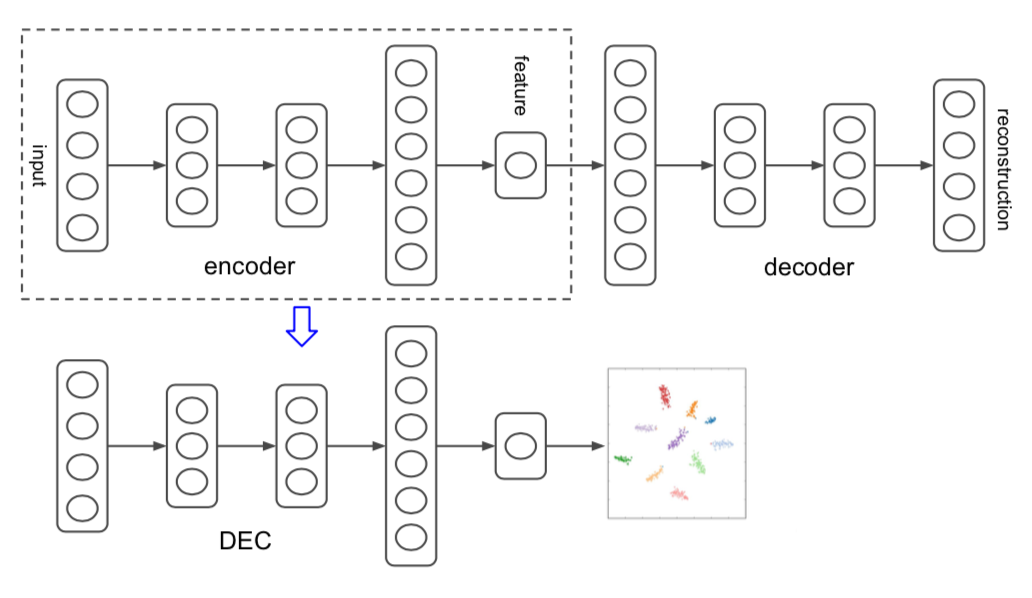
\includegraphics[width=12cm]{DAEar} 
\caption{Deep Auto-Encoder Architecture}\cite{xie2016unsupervised}
\label{fig:deepencoder}
\end{figure}  

Figure \ref{fig:deepencoder} shows a deep auto-encoder architecture used in both DEC and Deep Cluster, which is stacked by four auto-encoders with a structure of d-500-500-2000-10, where d is the original data dimension. Each auto-encoder inside uses a denoising criterion, by which can guide the learning of useful higher level representations\cite{vincent2010stacked}. To be concrete, input data $x$ is stochastically corrupted to $\tilde{x}$. The auto-encoder then maps it to y (via encoder $f_\theta$) and attempts to reconstruct $x$ via decoder $g_{\theta'}$ , producing reconstruction $\hat{x}$. Reconstruction error is measured by loss $\mathcal{L} (x, y)$.

\subsubsection{Deep Embedded Clustering}
Deep Embedded Clustering is proposed by \cite{xie2016unsupervised}, which firstly initializes parameter with deep auto-encoder and then optimizes parameter by minimizing the Kullback-Leibler(KL) divergence loss between a soft assignment $q_i$ and  an auxiliary target distribution $p_i$ ,where the $q_i$ is the similarity between embedded point $z_i$ and centroid $\mu_i$ computed with Student's t-distribution. 

\begin{equation}
\large
L=KL(P\|Q)=\sum\limits_i\sum\limits_jp_{ij}\log\frac{p_{ij}}{q_{ij}}
\end{equation}
The choice of  $p_i$ in the method is defined as:
\begin{equation}
\large
p_{ij}=\frac{q^2_{ij}/f_i}{\sum_j'q^2_{ij'}/f_{j'}}
\end{equation}
where $f_j=\sum_iq_{ij}$ are soft cluster frequencies.\\
Thus, cluster centroid $\mu_j$ and deep auto-encoder parameter $\theta$ can be optimized simultaneously using Stochastic Gradient Descent (SGD) with momentum. The gradients $\partial{L}/\partial{z_i}$ is computed to fed the deep auto-encoder and then by conducting standard back-propagation, parameter gradient $\partial{L}/\partial{z_i}$ in deep auto-encoder can be obtained. The stop criteria is set as when less than $tol\%$ of points change cluster assignment between two consecutive iterations.
\subsubsection{DeepCluster}
DeepCluster is proposed by \cite{tian2017deepcluster}, which build a framework where deep auto-encoder and clustering method are combined together. Specifically, in a single iteration, the latent feature representation is simultaneously used to reconstruct $\hat{x}$ as well as  conduct clustering, which is formulated as:
\begin{equation}
\begin{split}
&\min: \,\|{\textbf{X}}-\hat{\textbf{X}}\|_F^2+\lambda*{\mathcal{G}}_W(\textbf{Y}) \\
&s.t.  \,\,\,\,\,\,\,\,\, \textbf{Y}=f_{\theta_1}(\textbf{X})
\end{split}
\label{ref:deepEq}
\end{equation}
where $\textbf{X}$ is original feature representation and $\hat{\textbf{X}}$ is the reconstruction of deep auto-encoder. $\mathcal{G}_w(\textbf{Y})$ represent any specific clustering objective function such as K-means. $\textbf{Y}$ is a dummy variable that equals to latent feature representation. $\lambda$ defines the extent that clustering objective is weighted. \\
Since each layer is activated by non-linear function, object function is not convex, because of which optimization cannot be conducted directly with gradient-based methods. Instead, DeepCluster adopt ADMM to optimize it. Eq.(\ref{ref:deepEq}) can be derived to augmented Lagrangian as:

\begin{equation}
\large
  \mathcal{L}_\rho(\theta,\textbf{Y},\textbf{U},w)=\|\textbf{X}-\hat{\textbf{X}}\|^2_F+\lambda*\mathcal{G}_W(\textbf{Y})+\frac{\rho}{2}\|\textbf{Y}-f_{\theta_1}(\textbf{X})+\textbf{U}\|^2_F
\end{equation}
where $\textbf{U}$ is a scaled dual variable and $\rho > 0$ is the penalty parameter, which controls how close between $\textbf{Y}$ and $f_{\theta_1} (\textbf{X})$. We denotes auto-encoder parameter $\theta=\{\theta_1,\theta_2\}$, where $\theta_1$ indicates encoder parameter and $\theta_2$ indicates decoder parameter. To optimize $\theta$, we actually optimize $\|\textbf{X}-\hat{\textbf{X}}\|^2_F+\frac{\rho}{2}\|\textbf{Y}-f_{\theta_1}(\textbf{X})+\textbf{U}\|^2_F$ as the second part is independent from auto-encoder when clustering method is given. The function is non-convex as the first part is reconstruction error, which brings difficulties in proving its global convergence. However, experiments show that this method can converge to a good local minima when value $\rho$ is properly chosen(e.g.  $\rho=1$)\cite{tian2017deepcluster}.This method is flexible because $\mathcal{G}_w(\textbf{Y})$ could be any specific clustering algorithm. In our project, k-Means and GMM will be embedded in the framework. 
\subsection{Clustering Validation}
In the case of unsupervised learning it is required to validate the number of clusters due to lack of labels. There are two methods that can be used which help to find the appropriate number of clusters.

\subsubsection{Elbow Method}
In this method, the percentage of variance explained is expressed as a function of the number of clusters and plotted against the said number of clusters. The plot results in a curve with a knee and the cluster number corresponding to the knee is chosen as the appropriate value. As shown in Figure \ref{fig:nCluster} the elbow is at about k = 3, thus 3 is the optimal number of clusters. 
\begin{figure}[H]
	\centering
	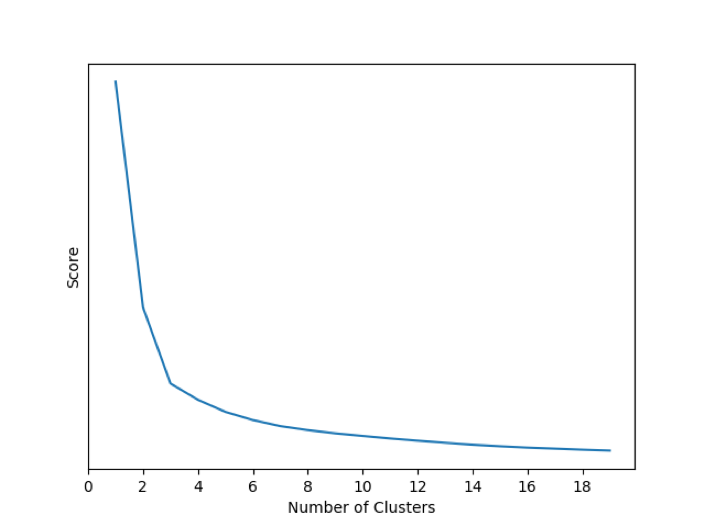
\includegraphics[height=3in]{nCluster}
	\caption[]{Elbow Curve}
	\label{fig:nCluster}
\end{figure}

\subsubsection{Silhouette Plots}
In this method, the separation distance between the clusters are measured. The plots show how close every point in one cluster is to every point in the other clusters. The average Silhouette coefficient calculated for the chosen number of clusters should be as close to 1 as possible. Also, no point in the clusters should have their Silhouette coefficient negative as it means that the said point has been wrongly classified. This means that the chosen number of clusters is not appropriate to describe the dataset. The thickness of the plots can also help identify the optimal number of clusters. Similar thickness plots are desired in addition to the above mentioned non-negative points.

\begin{figure}[H]
\centering
	\begin{subfigure}{.5\textwidth}
 	 \centering
  	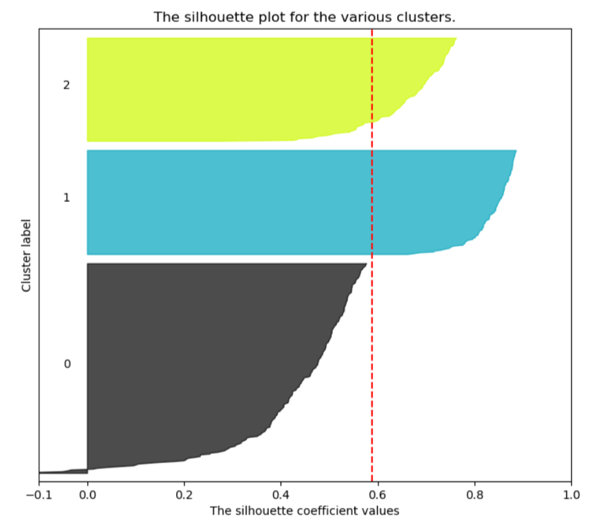
\includegraphics[height=2.5in]{spk3}
  	\caption{k=3}
 	 \label{fig:sub1}
	\end{subfigure}%
	\hfill
	\begin{subfigure}{.5\textwidth}
  	\centering
  	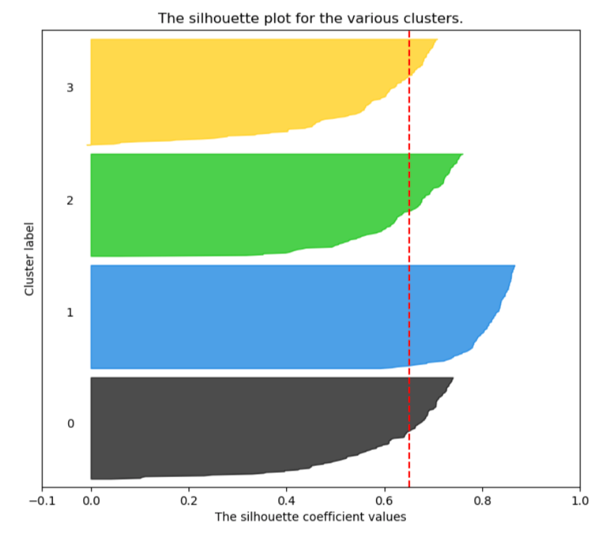
\includegraphics[height=2.5in]{spk4}
  	\caption{k=4}
  	\label{fig:sub2}
	\end{subfigure}
\caption{Silhouette Plots}
\label{fig:test}
\end{figure}


In Figure \ref{fig:sub1} and \ref{fig:sub2}, k = 3 and 4 respectively. The average silhouette coefficient for k = 4 is greater than k = 3. Also in Figure \ref{fig:sub1} there are points which have negative values. Thus, in this case, k = 4 is the optimal number of clusters.
\section{Resources}
\subsection{Hardware}
The applications will run on our own computer. The configurations are:
\begin{description}
\item[$\bullet$ ] MacBook Pro (13-inch, 2017, Two Thunderbolt 3 ports)
\item[$\bullet$ ]Processor 2.3 GHz Intel Core i5
\item[$\bullet$ ]Memory 8 GB 2133 MHz LPDDR3
\item[$\bullet$ ]Intel Iris Plus Graphics 640 1536 MB
\end{description}

\subsection{Software}

\begin{description}
\item[$\bullet$ ] Python 3.6
\item[$\bullet$ ] Keras 
\item[$\bullet$ ] Tensorflow
\item[$\bullet$ ] Anaconda(Jupyter Notebook)
\end{description}
\subsection{Roles \& Responsibilities}
\begin{table}[H]
\centering
	 \begin{tabular}{ | p{4cm}<{\centering} | p{4cm}<{\centering}|p{4cm}<{\centering}|}
	\hline
	\textbf{Name} & \textbf{Role} & \textbf{Responsibility} 
	\\ \hline
	\textbf{Min Jeong Oh} & Project manager, NLP analyst & Develop schedules, plan resources, monitor progress / text data feature engineering 
\\ \hline
	\textbf{Hongjin Qian} & NLP analyst, Admin & Text data feature engineering /Book meeting rooms
	\\ \hline
	\textbf{Luca Fu} & NLP analyst & Text data feature engineering	
	\\ \hline
	\textbf{Prerona Majumder} & ML analyst & Develop clustering model
	\\ \hline
	\textbf{Sheng Yuan} & ML analyst & Develop clustering model
	\\ \hline
	\end{tabular}
	\caption{Role and Responsibility}
\end{table}

\section{Expected Outcomes}
\subsection{Project Deliverables}
Report: This report will include the algorithm which the model applied. In addition, the whole process of this project will be shown in the report.\\
Source code: provide the source code using one program language.\\
Model: the model can distinguish different themes and give the rank of each theme which means that there are some themes are more important to a dataset. In addition, relatedness score between different themes will be given through this model.\\

\subsection{Implications}
Our role in the project is to build an unsupervised clustering model for text data. Unlike   supervised learning methods, we are trying to make the machine learn about the various text documents, their features, similarities, and the differences among them without any well-labelled trained data. Not knowing the ‘correct answers (labels or categories)’ in advance makes the task challenging, but we can discover latent characteristics which would have not been captured by manually crafted categories.\\
 
The clusters and important features of each cluster such as key sentences, key words, and other metadata will be reviewed by the experts from the related domains such as financial or legal domain. They will examine the patterns of the features and determine whether each cluster actually mean anything. For example, The Royal Commission Round 4 is about the issues with Australians who live in remote and regional communities, which relate to farming finance, and interactions between Aboriginal and Torres Strait Islander people and financial services entities. However, there can be latent themes such as ‘poor financial advice’, ‘predatory lending’, or ‘dysfunctional cultures’ which can be discovered by the clustering method. \\

This project is for providing an important step in Notion’s current business to generate business intelligence from large text for their clients especially Australian financial institutions. We think the latent themes discovered by the model can be used by financial institutions when they make strategic decisions like targeting specific groups of customers with specific products. Moreover, we expect this method can be extended to other business areas as a tool to discover customer behaviour and analyse market trends. \\



\section{Milestones / Schedule}
\begin{table}[H]
\centering
	 \begin{tabular}{ | p{2cm}<{\centering} | p{4cm}<{\centering}|p{3cm}<{\centering}| p{2cm}<{\centering} | p{2cm}<{\centering} | p{2cm}<{\centering} |}
	\hline
	\textbf{Milestone} & \textbf{Tasks} & \textbf{Start Date} &\textbf{Duration} &\textbf{End Date} 
	\\ \hline
	&Design Work Plan & 8/8/2018 &1& 8/9/2018
 	\\ \hline
	&Research & 8/10/2018 & 9 & 8/19/2018
	\\ \hline
	Y&Proposal Report&8/18/2018&13&8/31/2018
	\\ \hline
	&Build Environment&9/1/2018&4&9/5/2018
	\\ \hline
	&Development&9/6/2018&24&9/30/2018
\\ \hline
	&Testing&9/18/2018&12&9/30/2018
	\\ \hline
	Y&Progress Report Due&9/10/2018&25&10/5/2018
\\ \hline
	&Deployment&10/6/2018&8&10/14/2018
	\\ \hline
	&Documentation&10/15/2018&6&10/21/2018
	\\ \hline
	Y&Final Presentation&10/21/2018&8&10/29/2018
\\ \hline
	Y&Final Report (thesis)&10/18/2018&11&10/29/2018
\\ \hline
	\end{tabular}
	\caption{Schedule Table}
\end{table}


\begin{figure}[H] 
\centering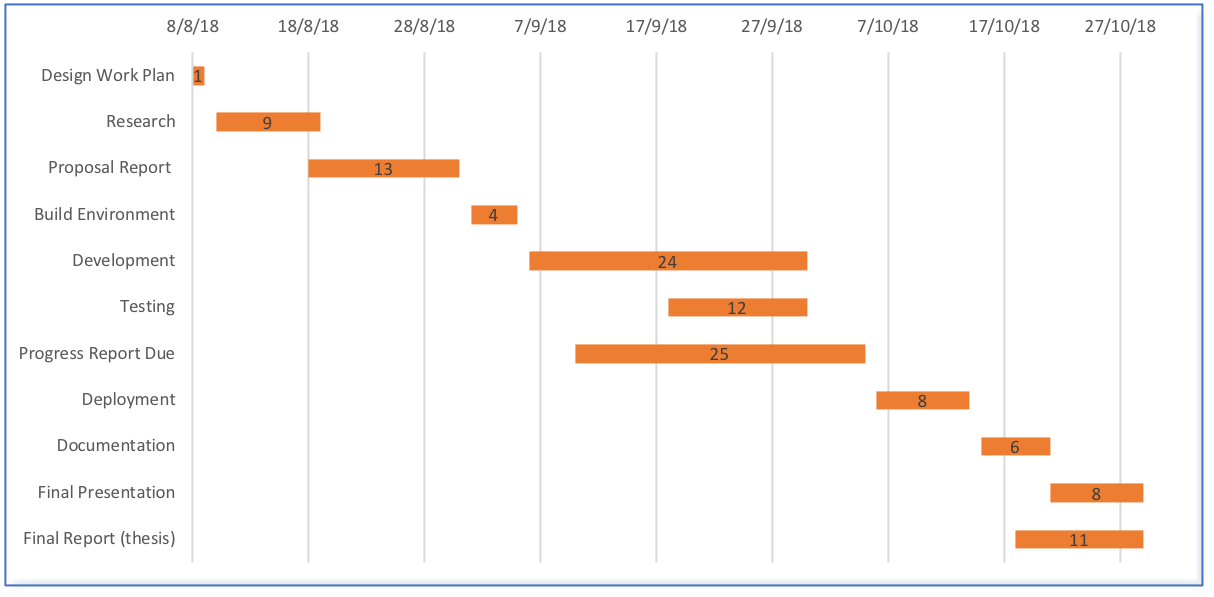
\includegraphics[width=12cm]{GanttChart} 
\caption{Project Gantt Chart}
\end{figure}  

\begin{description}
\item[$\bullet$ ] Design Work Plan: This project started in 08/08/2018. At first, a plan  about the whole project  which includes the duration of whole plan, start data of each stage and so on should be made.
\item[$\bullet$ ] Research : In this stage, we’ve conducted background research as well as method research. By the end of this stage, the major deliverables are literature reviews and background research.
\item[$\bullet$ ] Proposal Report : it is the milestone of the project. In terms of proposal report, it will focus on methodologies outcome and schedule.
\item[$\bullet$ ] Build environment: setting up the basis environment like python, IDE, API or some packages.
\item[$\bullet$ ] Development: comparing different models like Deep Neural Network Clustering Gaussian Mixture clustering. The main deliverable is   an algorithm to do the themes clustering and find the relationship among them.
\item[$\bullet$ ] Testing: Testing the program will cover the most time of development. it includes unit testing Integration testing and system testing. in each part of testing, the advantages and disadvantages of each model should be recorded.
\item[$\bullet$ ] Progress Report :it is the milestone of the project. this report will describe the progress of the project and what gonna do in the following stages.
\item[$\bullet$ ] Deployment: the deliverable of this stage is a program that easy to use instead of an simple model.
\item[$\bullet$ ] Documentation: in this stage, some instructions will be provided. the instructions includes some readable features, the rank and so on.
 \item[$\bullet$ ] Final Presentation and Final Report: Both final presentation and report are the milestone of the project. Presentation will talk about what have done about the project and the outcomes.  In terms of the final report, it will illustrate more details about the method used and compared.
\end{description}


\cleardoublepage
\bibliographystyle{apacite}
\bibliography{Proposal}
\end{document}
